\documentclass[11pt,a4paper]{article}

\usepackage[T1]{fontenc}
\usepackage[utf8]{inputenc}
% babel-spanish no está instalado en este sistema; se renombran a mano los
% rótulos automáticos para no depender de él.
\renewcommand{\contentsname}{Índice}
\renewcommand{\figurename}{Figura}
\renewcommand{\tablename}{Tabla}
\renewcommand{\abstractname}{Resumen}
\renewcommand{\refname}{Referencias}
\usepackage{amsmath,amssymb}
\usepackage{graphicx}
\usepackage{booktabs}
\usepackage{geometry}
\usepackage{xcolor}
\usepackage{hyperref}
\usepackage{caption}

\geometry{margin=2.4cm}
\hypersetup{colorlinks=true, linkcolor=blue!55!black, urlcolor=blue!55!black,
            citecolor=blue!55!black}

\graphicspath{{../resultados/images/}}

\newcommand{\ket}[1]{\lvert #1 \rangle}
\newcommand{\bra}[1]{\langle #1 \rvert}
\newcommand{\gm}{\mathfrak{g}}

\title{\textbf{Robustez de CD-ADAPT-VQE en qutrits frente a barren plateaus}\\[0.4em]
\large Informe técnico de la exploración numérica}
\author{Documento de trabajo --- grupo de investigación}
\date{\today}

\begin{document}
\maketitle

\begin{abstract}
\noindent
Este informe documenta una exploración numérica sobre CD-ADAPT-VQE aplicado a
Max-3-Cut en qutrits, con dos objetivos: (i) poner a prueba la afirmación de
que el pool contradiabático es robusto frente a \emph{barren plateaus}, y (ii)
evaluar qué cambia si los conmutadores que generan el pool se descomponen en la
base de Gell-Mann en vez de la de momento angular.

Se reporta tanto lo que funcionó como lo que no. Los resultados principales
son: el paisaje de optimización \emph{sí} es rugoso y los reinicios aleatorios
quedan atrapados en mínimos locales, pero ADAPT los evita por completo gracias
al reciclaje de parámetros; y la reformulación en base de Gell-Mann produce
generadores hermíticos por construcción y un pool $\sim$20\,\% más chico, pero
converge claramente peor. Se detallan las validaciones realizadas, un error
encontrado y corregido en la implementación, una predicción propia que resultó
equivocada, y las limitaciones que impiden generalizar las conclusiones.
\end{abstract}

\tableofcontents

\section{Contexto y objetivo}

CD-ADAPT-VQE construye el ansatz variacional de a un operador por vez,
eligiéndolo de un \emph{pool} generado por los conmutadores anidados del
Hamiltoniano adiabático. La afirmación que se quería poner a prueba es que, en
el caso qudit, ese pool es robusto frente a los efectos de \emph{barren
plateau}.

La estrategia es el análogo, para Max-3-Cut sobre qutrits, del experimento de
Grimsley \emph{et al.} (\emph{npj Quantum Information} \textbf{9}, 19, 2023),
que muestra que ADAPT-VQE es insensible a paisajes rugosos y mesetas.

\subsection{El problema}

El Hamiltoniano de costo para Max-3-Cut sobre $n$ qutrits (espín 1) es
\begin{equation}
H_C \;=\; \sum_{(i,j)\in E}\Big[ J_z^{(i)}J_z^{(j)} - 2\big((J_z^{(i)})^2+(J_z^{(j)})^2\big) + 3\,(J_z^{(i)})^2 (J_z^{(j)})^2 \Big],
\label{eq:HC}
\end{equation}
y el Hamiltoniano de mezcla
\begin{equation}
H_M \;=\; -\sum_{j} \tilde X_j, \qquad
\tilde X = J_z^2 + \sqrt{2}\,J_x = \begin{pmatrix}1&1&0\\1&0&1\\0&1&1\end{pmatrix},
\label{eq:HM}
\end{equation}
cuyo estado fundamental es la superposición uniforme
$\ket{\psi_0} = 3^{-n/2}\sum_x \ket{x}$, con autovalor $-2n\omega_0$.

Con la convención de la ecuación~\eqref{eq:HC}, cada arista \emph{cortada}
(extremos de distinta clase) aporta $-2$ y cada arista monocromática aporta
$0$. Por lo tanto $|E_0|/2$ es el número máximo de aristas cortables, lo que da
una verificación independiente de cualquier solución decodificada.

\subsection{La instancia estudiada y qué significa su solución}

Los experimentos se hacen sobre el grafo de la Fig.~1a del paper, de seis
vértices y diez aristas:
\begin{equation}
E = \{(1,2),(1,3),(1,4),(1,5),(2,4),(2,6),(3,4),(3,6),(4,5),(5,6)\},
\end{equation}
con secuencia de grados $(4,4,3,3,3,3)$ y $E_0 = -20$. La identificación con la
instancia~1 de la Tabla~I del paper se verificó reproduciendo sus cuatro filas:
razón de aproximación a tres decimales \emph{y} número exacto de parámetros de
parada coinciden en los cuatro grafos de comparación.

Una arista está \emph{cortada} si sus extremos quedan en clases distintas, y
Max-3-Cut consiste en maximizar cuántas lo están. Si un grafo admite una
coloración propia con tres colores, todas las aristas se cortan. El de la
Fig.~1a la admite, lo que se verificó por dos vías independientes: por el
espectro exacto ($|E_0|/2 = 10$ aristas cortables, que es el total) y por
enumeración de las $3^6=729$ coloraciones (máximo $10/10$, alcanzado por doce
coloraciones distintas, en acuerdo con la degeneración del fundamental).

La solución hallada reparte los vértices en las clases $\{2,3,5\}$, $\{1,6\}$ y
$\{4\}$, ninguna de las cuales contiene una arista interna --- son conjuntos
independientes ---, de modo que las diez aristas quedan entre clases distintas.

\subsection{Réplica de la figura del paper}

\begin{figure}[htbp]
\centering
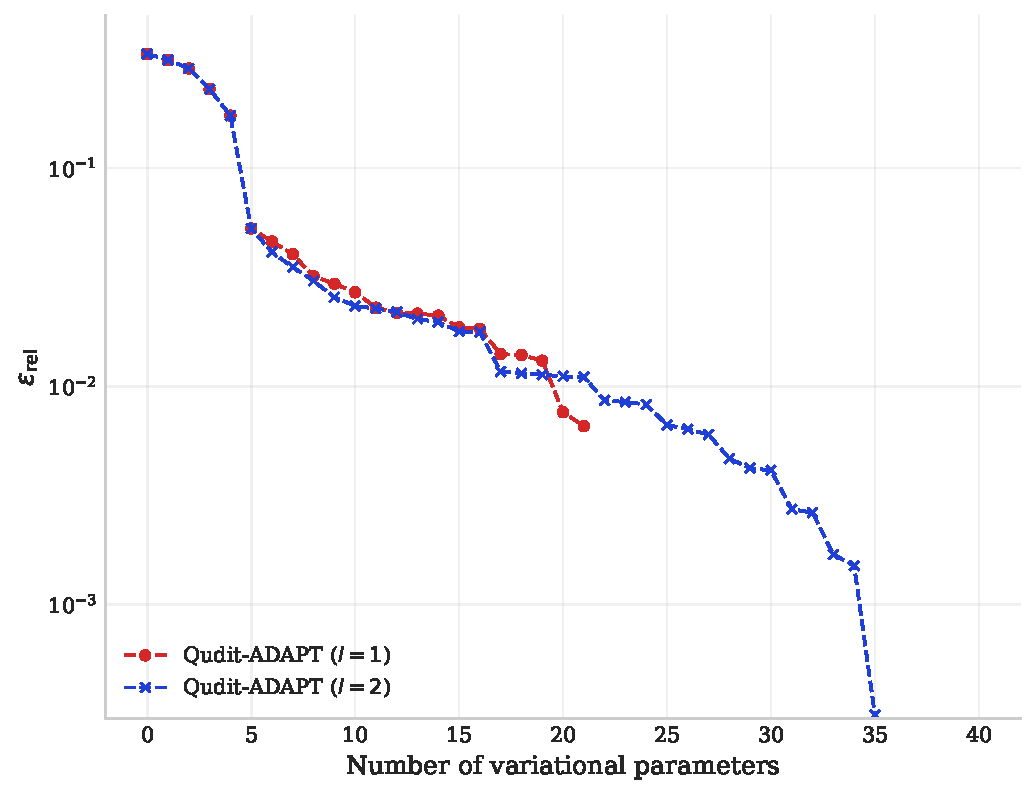
\includegraphics[width=0.68\textwidth]{replica_fig1a.pdf}
\caption{Réplica de la Fig.~1a: error relativo $\epsilon_{\rm rel}$ contra
número de parámetros variacionales, para los pools $\ell=1$ y $\ell=2$.}
\label{fig:replica}
\end{figure}

\begin{center}
\begin{tabular}{lrrrr}
\toprule
& \multicolumn{2}{c}{Este trabajo} & \multicolumn{2}{c}{Tabla I del paper} \\
\cmidrule(lr){2-3}\cmidrule(lr){4-5}
& $r$ & Parámetros & $r$ & Parámetros \\
\midrule
Qudit-ADAPT $\ell=1$ & 0.9934 & 21 & 0.993 & 21 \\
Qudit-ADAPT $\ell=2$ & 1.0000 & 40 & 0.999 & 40 \\
\bottomrule
\end{tabular}
\end{center}

Para $\ell=1$ la coincidencia es exacta, incluido el punto de parada por el
criterio de gradiente. Para $\ell=2$ este trabajo obtiene
$\epsilon_{\rm rel} = 3.2\times10^{-7}$ frente a $6.1\times10^{-4}$, unas dos
mil veces mejor con el mismo ansatz de cuarenta parámetros. La única diferencia
metodológica es el uso de gradiente analítico en lugar de diferencias finitas,
lo que sugiere que el valor de la Tabla~I para $\ell=2$ está limitado por la
convergencia del optimizador y no por la expresividad del ansatz.

\paragraph{Una observación sobre la métrica.} Con $\ell=1$ y 21 parámetros la
energía \emph{no} ha convergido ($\epsilon_{\rm rel}=6.6\times10^{-3}$), pero el
estado de la base computacional más probable ya es una coloración
\emph{exactamente} óptima, con probabilidad $0.47$. En optimización combinatoria
lo que importa es que la solución correcta sea el resultado más probable de
medir, y eso ocurre bastante antes que la convergencia energética. Es una
diferencia de fondo con el caso molecular, donde el observable de interés es la
energía misma.

\section{Metodología}

\subsection{El experimento}

Cada vez que ADAPT agrega un operador, el ansatz de $k$ parámetros se
re-optimiza desde tres tipos de punto inicial distintos:

\begin{center}
\begin{tabular}{lll}
\toprule
Estrategia & Punto inicial & Qué representa \\
\midrule
Reciclada & $(\boldsymbol\theta^*_{k-1},\, 0)$ & el algoritmo real \\
Fría & $\boldsymbol\theta = 0$ & reinicia el estado a $\ket{\psi_0}$ en cada paso \\
Aleatoria ($\times 20$) & $\theta_j \sim \mathcal U(-\pi,\pi)$ & un ansatz de tamaño fijo sin información previa \\
\bottomrule
\end{tabular}
\end{center}

De cada instancia aleatoria se registra \textbf{sólo el óptimo final}, no la
trayectoria. Ésa es la diferencia importante: cada marca en las figuras es
entonces un mínimo del paisaje donde efectivamente terminó una optimización, de
modo que cada columna muestra la \emph{estructura de mínimos locales} que ve un
ansatz de ese tamaño.

La curva fría es el contrafactual clave: usa exactamente la misma secuencia de
operadores y el mismo pool, y lo único que cambia es el punto de partida de la
optimización.

\subsection{Implementación y validación}

El motor numérico reimplementa el bucle de CD-ADAPT-VQE en
\texttt{numpy}/\texttt{scipy.sparse} con \textbf{gradiente analítico} obtenido
por retropropagación sobre el producto de exponenciales:
\begin{equation}
\frac{\partial E}{\partial\theta_j} = 2\,\mathrm{Im}\,\bra{\sigma_j} A_j \ket{\phi_j},
\qquad
\ket{\phi_j} = U_j\cdots U_1\ket{\psi_0},\quad
\ket{\sigma_j} = R_j^\dagger H_C\ket{\psi},
\end{equation}
con $R_j = U_m\cdots U_{j+1}$ y $\sigma_{j-1} = U_j^\dagger\sigma_j$. Esto
cuesta $O(m)$ productos matriz-vector para las $m$ derivadas, en vez de
$O(m^2)$ por diferencias finitas.

La elección es deliberada: en un estudio sobre gradientes no se quiere que el
optimizador se detenga por ruido de diferencias finitas en vez de por la
geometría real del paisaje.

Se realizaron las siguientes validaciones, todas superadas:

\begin{center}
\begin{tabular}{lll}
\toprule
Qué se verificó & Contra qué & Resultado \\
\midrule
Gradiente analítico & diferencias finitas centradas & $4\times10^{-9}$ \\
Energía del ansatz & \texttt{qutip} (código original) & $9\times10^{-16}$ \\
Pool contradiabático & \texttt{cd\_adapt\_vqe\_algorithm\_profundo} & idéntico elemento a elemento \\
Curva reciclada & \texttt{energy\_trace} del original & $6\times10^{-11}$ \\
Generadores del ansatz & reconstrucción desde la etiqueta & $0$ exacto \\
\bottomrule
\end{tabular}
\end{center}

Un detalle que apareció y conviene documentar: los índices de operador
seleccionados difieren de los del código original. No es un error. En grafos
simétricos varios operadores empatan en el gradiente hasta $\sim10^{-15}$, y
\texttt{argmax} rompe el empate según el último bit de precisión. Los
operadores elegidos son equivalentes por simetría y las trazas de energía
coinciden.

\section{Resultados: barren plateaus}

\subsection{Caso principal}

\begin{figure}[htbp]
\centering
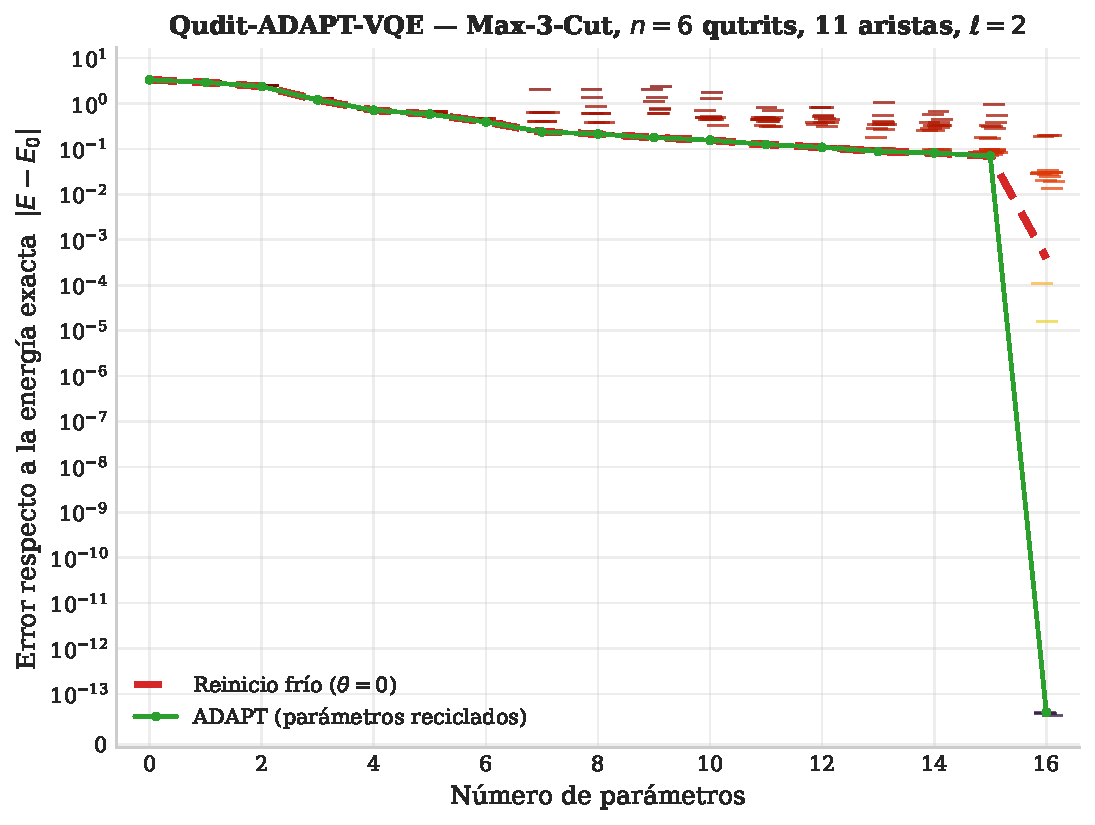
\includegraphics[width=0.72\textwidth]{bp_landscape_n6_l2_grafo2.pdf}
\caption{$n=6$ qutrits, 11 aristas, pool $\ell=2$. Cada marca horizontal es el
óptimo final de una de 20 instancias con parámetros iniciales aleatorios. La
curva verde es ADAPT con parámetros reciclados; la roja punteada reinicia en
$\theta=0$ en cada paso. A la derecha, el grafo con la solución Max-3-Cut
hallada: rojo son las aristas cortadas, gris punteado las monocromáticas.}
\label{fig:principal}
\end{figure}

Para el grafo de 11 aristas con $\ell=2$ ($E_0 = -18$, degeneración 180,
\emph{gap} espectral 2):

\begin{center}
\begin{tabular}{lr}
\toprule
& Error final $|E-E_0|$ \\
\midrule
ADAPT (parámetros reciclados) & $6.4\times10^{-14}$ \\
Reinicio frío ($\theta=0$) & $3.9\times10^{-4}$ \\
Aleatorios --- mejor de 20 & $5.7\times10^{-14}$ \\
Aleatorios --- \textbf{mediana} & $2.7\times10^{-2}$ \\
Aleatorios --- peor de 20 & $1.9\times10^{-1}$ \\
\bottomrule
\end{tabular}
\end{center}

Sólo \textbf{3 de 20} instancias aleatorias alcanzan $|E-E_0|<10^{-6}$. La
mediana queda $\sim10^{11}$ veces peor que ADAPT, y la dispersión del paisaje
(peor sobre mejor reinicio) llega a $3\times10^{12}$.

La lectura es directa: el paisaje \textbf{sí} está lleno de mínimos locales
--- no es que el problema sea fácil --- pero ADAPT no los ve.

\subsection{Por qué la caída es abrupta: \emph{burrowing}}

En la figura~\ref{fig:principal} el error cae doce órdenes de magnitud en un
solo paso, de $k=15$ a $k=16$. Se verificó que esto es correcto y no un
artefacto numérico.

\paragraph{El mecanismo.} Sea $E_k$ el paisaje de $k$ parámetros y
$\boldsymbol\theta^*_k$ un mínimo local suyo. Al agregar un operador con
$\theta_{k+1}=0$ se tiene $E_{k+1}(\boldsymbol\theta,0) = E_k(\boldsymbol\theta)$,
de modo que el paisaje viejo queda embebido como una rebanada del nuevo. En el
punto de partida,
\begin{equation}
\frac{\partial E_{k+1}}{\partial\theta_i}\bigg|_{(\boldsymbol\theta^*_k,0)} = 0 \;\;(i\le k),
\qquad
\frac{\partial E_{k+1}}{\partial\theta_{k+1}}\bigg|_{(\boldsymbol\theta^*_k,0)} = i\bra{\psi_k}[H_C,A_{k+1}]\ket{\psi_k} \neq 0 ,
\end{equation}
donde la segunda es precisamente el gradiente que ADAPT maximiza al elegir el
operador. Es decir: lo que era un mínimo local en $k$ dimensiones deja de serlo
al embeberlo en $k+1$ --- se convierte en un punto de silla con una dirección
cuesta abajo garantizada.

De ahí el nombre: en vez de \emph{escalar} la barrera que rodea al mínimo
local, el algoritmo \emph{excava} por una dimensión que antes no existía. Se
siguen dos consecuencias: la energía óptima es monótona no creciente, y los
mínimos locales del ansatz de tamaño fijo nunca se visitan, porque ADAPT jamás
arranca desde un punto arbitrario de ese paisaje.

\paragraph{Verificación.} El estado final satisface
\begin{equation}
\big\| P_{\rm gs}\ket{\psi}\big\|^2 = 1.0000000000 ,
\end{equation}
donde $P_{\rm gs}$ proyecta sobre el subespacio fundamental (180 veces
degenerado). El estado no está \emph{cerca} del fundamental: está
completamente dentro del subespacio, y el error $6.4\times10^{-14}$ es
precisión de máquina.

La razón de fondo es que Max-3-Cut tiene espectro discreto y estados
fundamentales exactamente alcanzables por un circuito finito. Esto lo distingue
del caso molecular de la figura original, donde el fundamental de FCI es
genéricamente irracional y la convergencia es asintótica. Aquí no hay
gradualidad posible: o el ansatz alcanza el subespacio o no lo alcanza.

Como respaldo adicional, \textbf{8 de los 16 parámetros optimizados son
múltiplos exactos de $\pi/2$} (cuatro valen exactamente $\pi/2$ y cuatro
exactamente $0$), lo que corresponde a rotaciones discretas exactas y no a
valores ajustados numéricamente. Nótese también que cuatro parámetros son
esencialmente nulos: el ansatz tiene $\sim$12 parámetros \emph{activos} de los
16 nominales.

\paragraph{Alcance del argumento.} El \emph{burrowing} no es un teorema de
optimalidad global. Garantiza mejora monótona y escape de los mínimos del
ansatz anterior, pero el algoritmo puede converger a un punto subóptimo si el
gradiente de todo el pool se anula lejos del fundamental. El caso $\ell=1$ que
sigue lo ilustra.

\subsection{Caso con pool reducido ($\ell=1$)}

\begin{figure}[htbp]
\centering
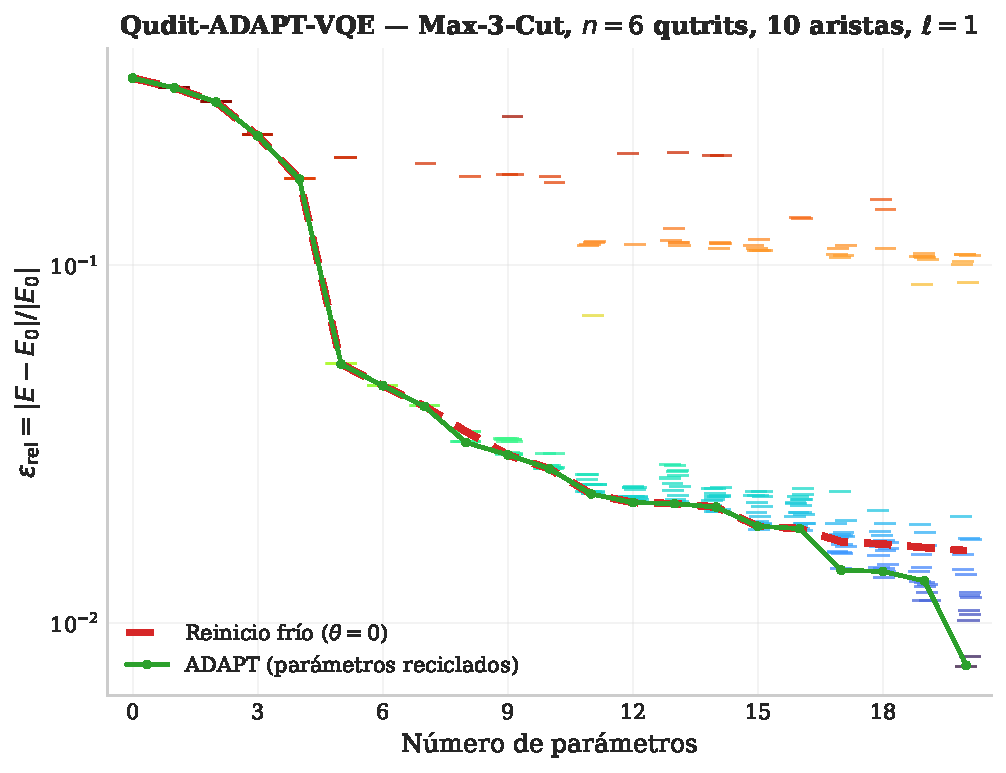
\includegraphics[width=0.72\textwidth]{bp_landscape_n6_l1_grafo1.pdf}
\caption{$n=6$ qutrits, 10 aristas, pool $\ell=1$ (sólo $O_1$). El algoritmo se
estanca en $1.5\times10^{-1}$, pero la nube de instancias aleatorias se
despliega en todas las columnas y la separación respecto de ADAPT es visible en
todo el rango.}
\label{fig:l1}
\end{figure}

Con el pool reducido ($E_0=-20$, degeneración 12) ADAPT llega a
$1.5\times10^{-1}$, la curva fría a $3.2\times10^{-1}$, y la mediana de los
reinicios aleatorios a $3.0\times10^{-1}$, con $0/20$ instancias por debajo de
$10^{-6}$. La solución decodificada corta las 10 aristas de 10, lo que se verifica contra
$|E_0|/2 = 10$.

Este caso muestra el límite del argumento: ADAPT sigue siendo mejor que
cualquier reinicio aleatorio, pero se estanca por \emph{limitación del pool},
no por el paisaje.

\subsection{Diagnóstico de gradientes}

\begin{figure}[htbp]
\centering
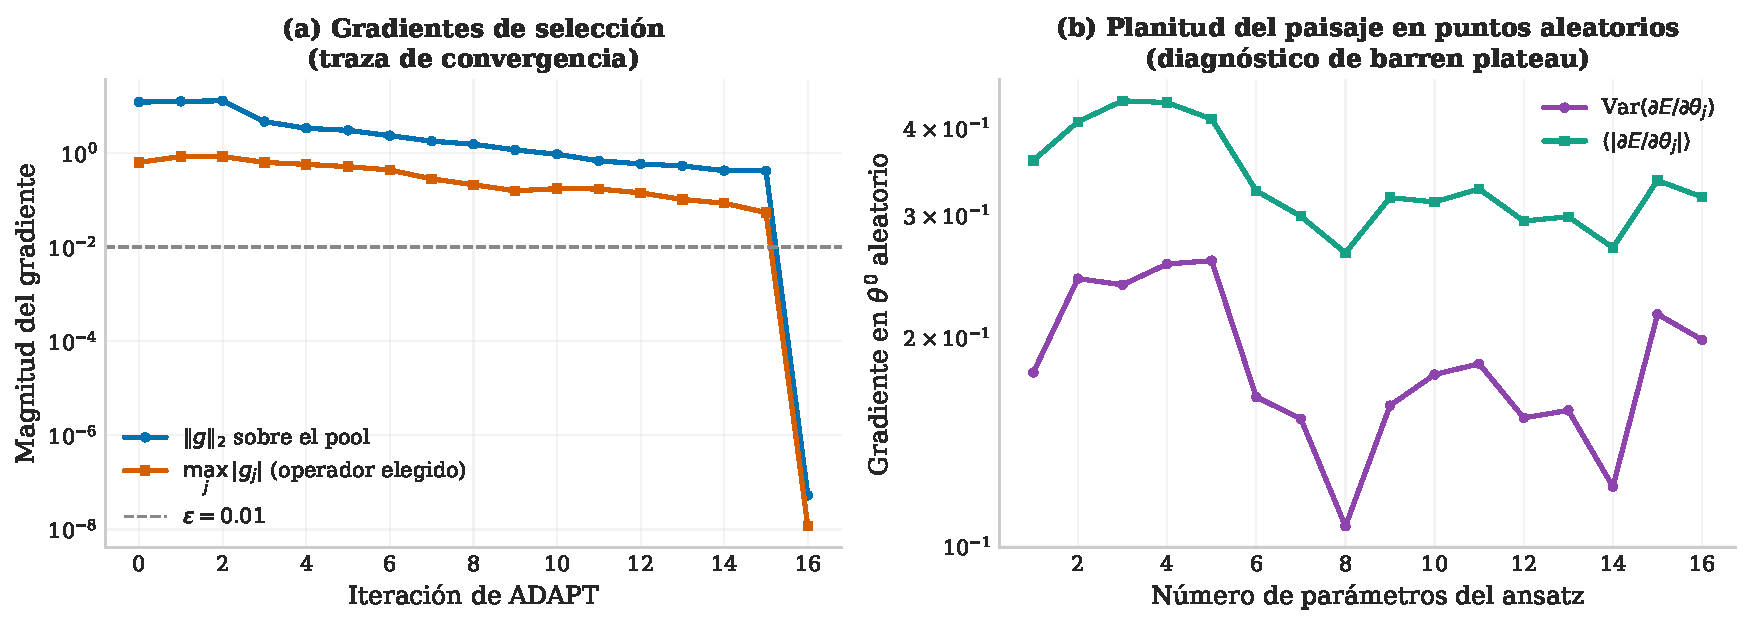
\includegraphics[width=\textwidth]{bp_gradientes_n6_l2_grafo2.pdf}
\caption{(a) Gradientes de selección a lo largo de la trayectoria de ADAPT.
(b) Varianza y magnitud media del gradiente evaluado en los mismos puntos
iniciales aleatorios, en función del tamaño del ansatz.}
\label{fig:grad}
\end{figure}

Conviene ser preciso sobre qué mide cada panel, porque es fácil sacar una
conclusión que los datos no sostienen.

El panel (a) muestra los gradientes de selección $|g_j| = |\bra{\psi_k}[H_C,A_j]\ket{\psi_k}|$
a lo largo de la propia trayectoria del algoritmo. Estos gradientes
\textbf{bajan}, pero eso no dice nada sobre \emph{barren plateaus}: bajan
porque el algoritmo se acerca al mínimo. Es una traza de convergencia.

El panel (b) es el diagnóstico pertinente. Un \emph{barren plateau} no es que
el gradiente baje cerca del óptimo, sino que el paisaje sea exponencialmente
plano \emph{en puntos de parámetros aleatorios}. Reevaluando el gradiente
exacto en los mismos $\boldsymbol\theta^0$ aleatorios del experimento:
\begin{center}
\begin{tabular}{lrrr}
\toprule
Caso & Var con 1 parám. & Var con $k_{\max}$ parám. & Ajuste log-lineal \\
\midrule
$\ell=2$, 11 aristas & $1.78\times10^{-1}$ & $1.98\times10^{-1}$ & $e^{-0.020\,k}$ \\
$\ell=1$, 10 aristas & $1.78\times10^{-1}$ & $1.76\times10^{-1}$ & $e^{-0.024\,k}$ \\
\bottomrule
\end{tabular}
\end{center}
No hay aplanamiento exponencial con la profundidad. Lo que atrapa a los
reinicios aleatorios son mínimos locales, no una meseta.

\subsection{Geometría: matriz de información cuántica de Fisher}

La QFIM,
$F_{ij} = 4\,\mathrm{Re}[\langle\partial_i\psi|\partial_j\psi\rangle - \langle\partial_i\psi|\psi\rangle\langle\psi|\partial_j\psi\rangle]$,
es de tamaño $k\times k$ con $k$ el número de parámetros variacionales, y
describe la geometría de la variedad que barre el ansatz. Se validó contra el
caso analítico $F_{11} = 4\,\mathrm{Var}(A)$ para un parámetro, con acuerdo a
$10^{-16}$.

Resultados: el rango es exactamente $k$ hasta 14 parámetros (cada operador
aporta una dirección nueva, sin redundancia), y sobre la familia de ciclos
$C_n$ con un ansatz de 8 operadores, el autovalor medio se mantiene
$\mathcal O(1)$ mientras el espacio de Hilbert crece 27 veces:

\begin{center}
\begin{tabular}{rrr}
\toprule
$n$ & $\dim\mathcal H$ & Autovalor medio \\
\midrule
3 & 27 & 0.857 \\
4 & 81 & 1.099 \\
5 & 243 & 0.968 \\
6 & 729 & 0.809 \\
\bottomrule
\end{tabular}
\end{center}

\paragraph{Advertencia sobre la interpretación.} Por órbita-estabilizador,
$\mathrm{rank}\,F(\theta) \le \min(k,\ \dim\gm - \dim\mathfrak{k})$, con
$\mathfrak k$ el estabilizador de $\ket{\psi_0}$. Por lo tanto un rango igual a
$k$ sólo establece la \emph{cota inferior} $\dim\gm - \dim\mathfrak k \ge k$:
significa que aún no se satura, y no constituye un cálculo del álgebra de Lie.

\subsection{Álgebra de Lie dinámica}

El DLA es la subálgebra de Lie real generada por los operadores del circuito,
$\gm = \langle iG_1,\dots,iG_M\rangle_{\rm Lie}$. Su relevancia proviene de la
teoría de Ragone \emph{et al.} (\emph{Nat. Commun.} \textbf{15}, 2024), que
liga la varianza de la función de costo con $\dim\gm$.

El cálculo es una clausura de Lie por Gram-Schmidt, sobre el espacio real de
matrices antihermíticas (donde el producto de Hilbert-Schmidt es real). Se
validó contra álgebras de dimensión conocida: $\{\sigma_x,\sigma_y\}\to 3$,
espín-1 $\{J_x,J_y,J_z\}\to 3$, generadores de $\mathfrak{su}(3)$ sin traza
$\to 8$, operadores que conmutan $\to 2$.

Sobre el ansatz que ADAPT genera realmente (familia de ciclos, $\ell=1$):

\begin{center}
\begin{tabular}{rrrrr}
\toprule
$n$ & $D=3^n$ & $\dim\mathfrak u(D)$ & Generadores distintos & $\dim\gm$ \\
\midrule
2 & 9 & 81 & 2 & 4 \\
3 & 27 & 729 & 8 & 169 \\
\bottomrule
\end{tabular}
\end{center}

La fracción de $\mathfrak u(D)$ sube de 4.9\,\% a 23.2\,\%, lo que apunta a
crecimiento exponencial más que polinomial. El cálculo para $n=4$ quedó
pendiente por costo computacional.

\paragraph{Dirección de la implicación.} Si se confirmara el crecimiento
exponencial, esto \emph{no} implica que ADAPT sufra \emph{barren plateaus}. La
implicación útil va en un solo sentido: $\dim\gm$ polinomial $\Rightarrow$ no
hay meseta. La recíproca no vale porque el teorema supone circuitos
suficientemente profundos, donde promediar sobre parámetros equivale a
promediar Haar sobre $G=e^{\gm}$; los circuitos de ADAPT son cortos,
estructurados y con parámetros reciclados, lejos de ese régimen.

\section{Reformulación en la base de Gell-Mann}

\subsection{Motivación}

El pool se construye tomando los \emph{términos individuales} de los
conmutadores anidados, así que depende de en qué base se los descomponga. En la
base de momento angular aparecen productos como $J_y^{(1)}J_z^{(1)}$ --- dos
ejes en el mismo sitio --- que no son hermíticos, y el algoritmo original los
hermitiza al final con $(O+O^\dagger)/2$.

Las matrices de Gell-Mann evitan ese paso, porque el álgebra cierra
linealmente: $[\lambda_a,\lambda_b] = 2i\sum_c f_{abc}\lambda_c$. Cada término
del conmutador queda como un producto de $\lambda$'s sobre sitios
\emph{distintos}, que conmutan y son hermíticas; multiplicado por $i$ el
generador es hermítico por construcción.

Escrito en esta base, el Hamiltoniano de costo es notablemente más compacto:
\begin{equation}
H_C\big|_{(i,j)} \;=\; \lambda_3^{(i)}\lambda_3^{(j)} + \lambda_8^{(i)}\lambda_8^{(j)} - \tfrac{4}{3}\mathbb{1},
\end{equation}
esto es \textbf{dos} términos de interacción por arista en vez de cuatro.
Además no tiene parte de un solo sitio: los términos locales de la
ecuación~\eqref{eq:HC} se absorben en la constante.

\subsection{Validación}

Como ambas bases generan el mismo espacio, los Hamiltonianos deben ser
idénticos; si no lo fueran, nada de la comparación sería válido.

\begin{center}
\begin{tabular}{ll}
\toprule
Verificación & Resultado \\
\midrule
$f_{abc}$ calculadas de las matrices vs.\ valores tabulados & exactas \\
Regla de producto $\lambda_a\lambda_b = \frac{2}{3}\delta_{ab}\mathbb1 + (d+if)_{abc}\lambda_c$ & $3\times10^{-16}$ \\
$H_M$, $H_C$ en Gell-Mann vs.\ implementación original & $\sim10^{-15}$ \\
Conmutador simbólico vs.\ conmutador matricial & $1\times10^{-15}$ \\
Hermiticidad del pool \emph{sin} hermitizar & $0$ exacto \\
\bottomrule
\end{tabular}
\end{center}

\paragraph{Un error encontrado y corregido.} La primera implementación evaluaba
el conmutador en $\lambda=0.5$. El código original mantiene $\lambda$ simbólico
(\texttt{sympy}), de modo que un término desaparece sólo si su coeficiente se
anula como polinomio; al evaluar numéricamente en un valor particular pueden
cancelarse términos por accidente. Con $\lambda=0.5$ el pool $\ell=2$ perdía 24
strings (888 en vez de 912). Se corrigió evaluando en dos valores genéricos y
tomando la unión.

\subsection{Comparación}

\begin{figure}[htbp]
\centering
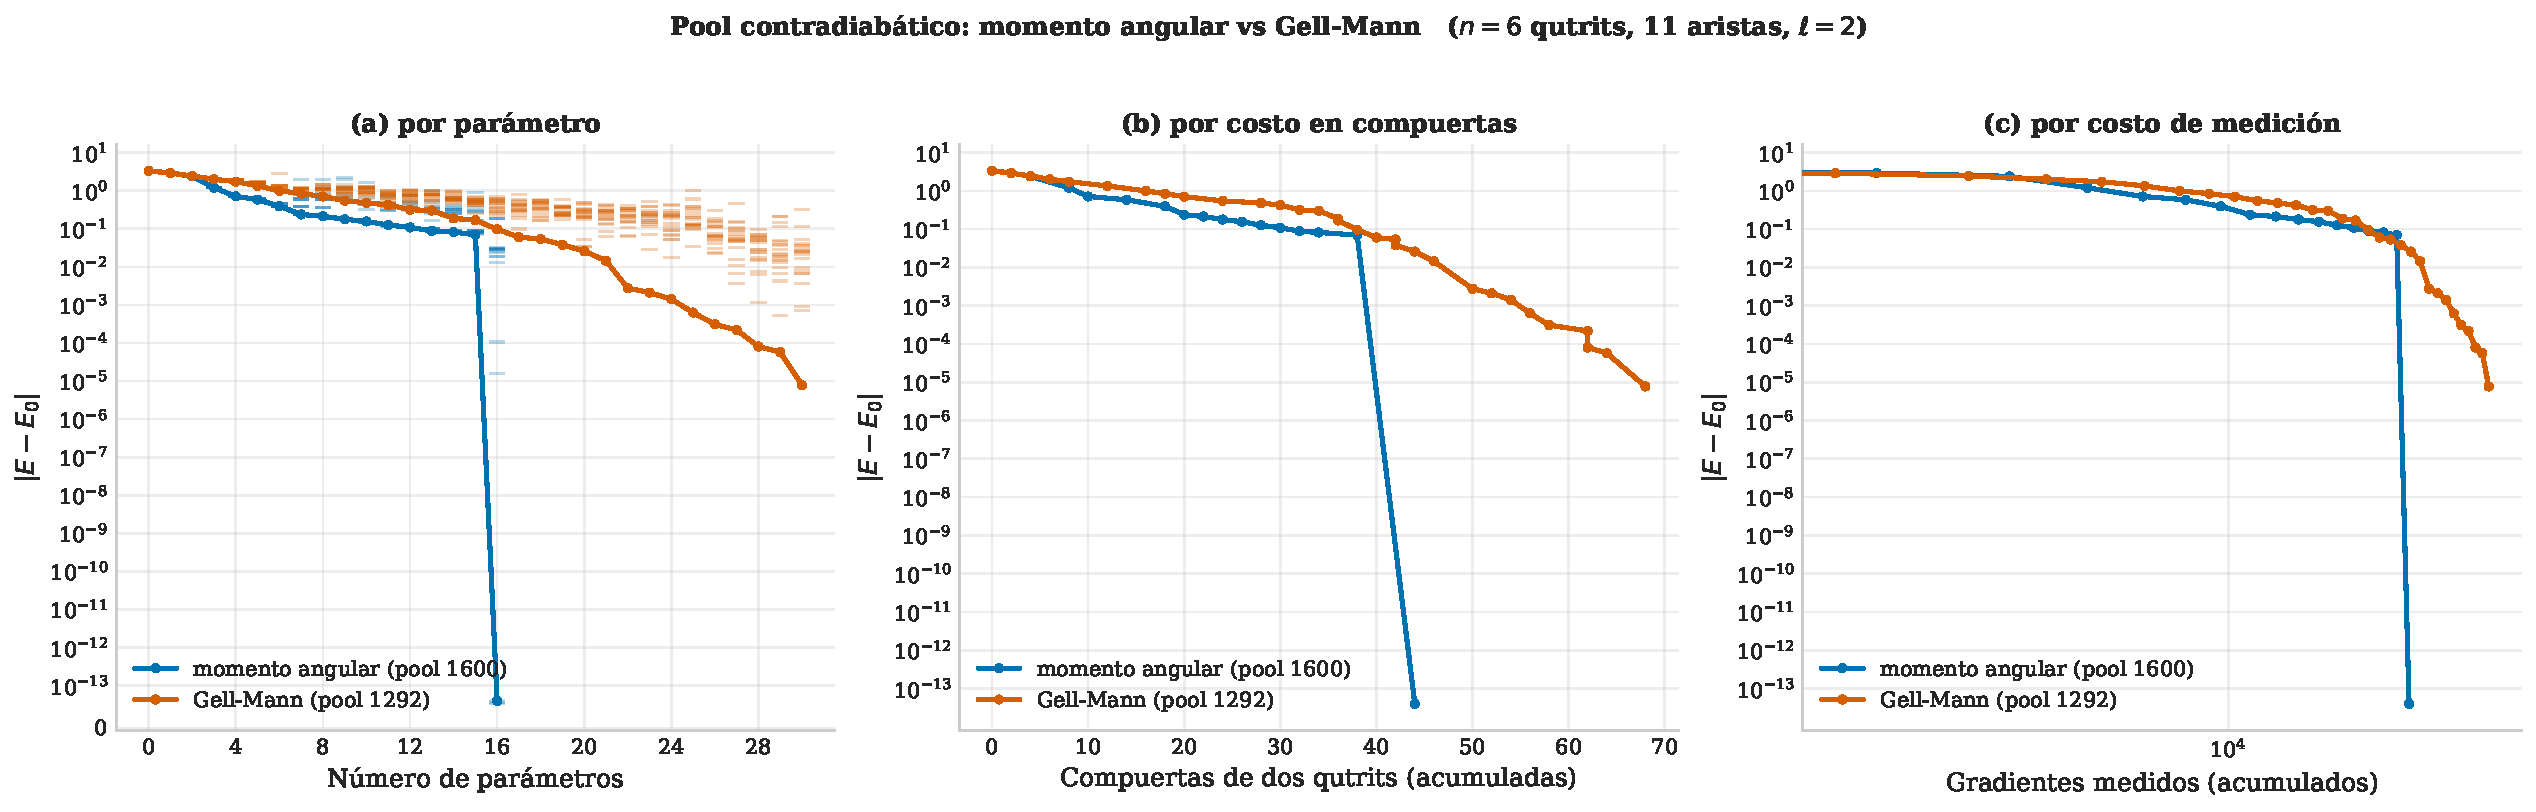
\includegraphics[width=\textwidth]{bp_pools_n6_l2_grafo2.pdf}
\caption{Comparación de pools sobre el mismo problema ($n=6$, 11 aristas,
$\ell=2$). (a) por parámetro; (b) por costo en compuertas entrelazantes;
(c) por costo de medición.}
\label{fig:pools}
\end{figure}

\paragraph{Sobre la métrica.} Comparar por número de parámetros es injusto
entre pools distintos, porque un pool con operadores de mayor peso baja más el
error por parámetro pero cada compuerta cuesta más. Un operador que actúa sobre
$w$ sitios se implementa con $\sim 2(w-1)$ compuertas de dos qutrits. Se
reportan además las \emph{mediciones de gradiente}, que en hardware suelen
dominar el costo: cada iteración de ADAPT evalúa el gradiente de todo el pool,
de modo que el total escala como $|{\rm pool}|\times n_{\rm iter}$.

\begin{center}
\begin{tabular}{lrrrrr}
\toprule
Base & Pool & Operadores & Error final & Compuertas & Mediciones \\
\midrule
Momento angular & 1600 & 16 & $6.4\times10^{-14}$ & 44 & 25\,600 \\
Gell-Mann & 1292 & 30 & $7.8\times10^{-6}$ & 68 & 38\,760 \\
\bottomrule
\end{tabular}
\end{center}

Para alcanzar $|E-E_0| < 10^{-2}$: momento angular necesita 25\,600 mediciones
y 44 compuertas; Gell-Mann, 28\,424 mediciones y 50 compuertas.

\subsection{Interpretación}

\textbf{A favor de Gell-Mann.} La hermiticidad es exacta sin ningún parche, lo
que hace la construcción más limpia teóricamente. Y el pool es un
$\sim$20\,\% más chico, lo que se traduce directamente en menos gradientes que
medir por iteración.

\textbf{En contra.} Converge claramente peor, en las tres métricas. La
explicación más plausible es que los operadores del pool angular son
$(O+O^\dagger)/2$ de monomios como $J_{z,i}^2J_{z,j}^2$, que en base de
Gell-Mann son \emph{compuestos}: cada uno es una suma de varios strings. Los
strings de Gell-Mann son los elementos atómicos, de modo que cada uno hace
menos trabajo por paso. Una descomposición más fina da un pool más chico y más
fácil de compilar, pero cada elemento es menos expresivo.

Se observa además que con $\ell=1$ el pool de Gell-Mann resulta 100\,\% de peso
2: no contiene rotaciones de un solo sitio, que son baratas y útiles en las
primeras iteraciones.

\paragraph{Una predicción propia que resultó equivocada.} Se anticipó que la
métrica de medición podía revertir la conclusión, dado que el pool de
Gell-Mann es más chico. No ocurre: el pool angular gana también ahí. Lo que sí
hace la métrica es \emph{estrechar} el margen considerablemente --- de ocho
órdenes de magnitud en el error final a sólo un 11\,\% más de mediciones para
precisión moderada.

\subsection{Conteo de compuertas en el conjunto nativo}

La comparación anterior usaba una métrica de costo genérica. Se rehízo con el
conjunto de compuertas del procesador universal de qudits con iones atrapados
de Ringbauer \emph{et al.} (\emph{Nat. Phys.} \textbf{18}, 1053, 2022), que es
la referencia de hardware del paper:
\begin{equation}
R^{(i,j)}(\theta,\varphi)=e^{-i\theta\sigma_\varphi^{(i,j)}/2},
\qquad
\mathrm{MS}^{(i,j)}(\theta,\varphi)=e^{-i\frac{\theta}{4}\left(\sigma_\varphi^{(i,j)}\otimes\mathbb1+\mathbb1\otimes\sigma_\varphi^{(i,j)}\right)^2},
\end{equation}
donde $(i,j)$ selecciona un \emph{par de niveles}. Una unitaria arbitraria de un
qudit se descompone en $\mathcal O(d^2)$ rotaciones de dos niveles vía Givens;
para $d=3$ bastan tres.

\begin{figure}[htbp]
\centering
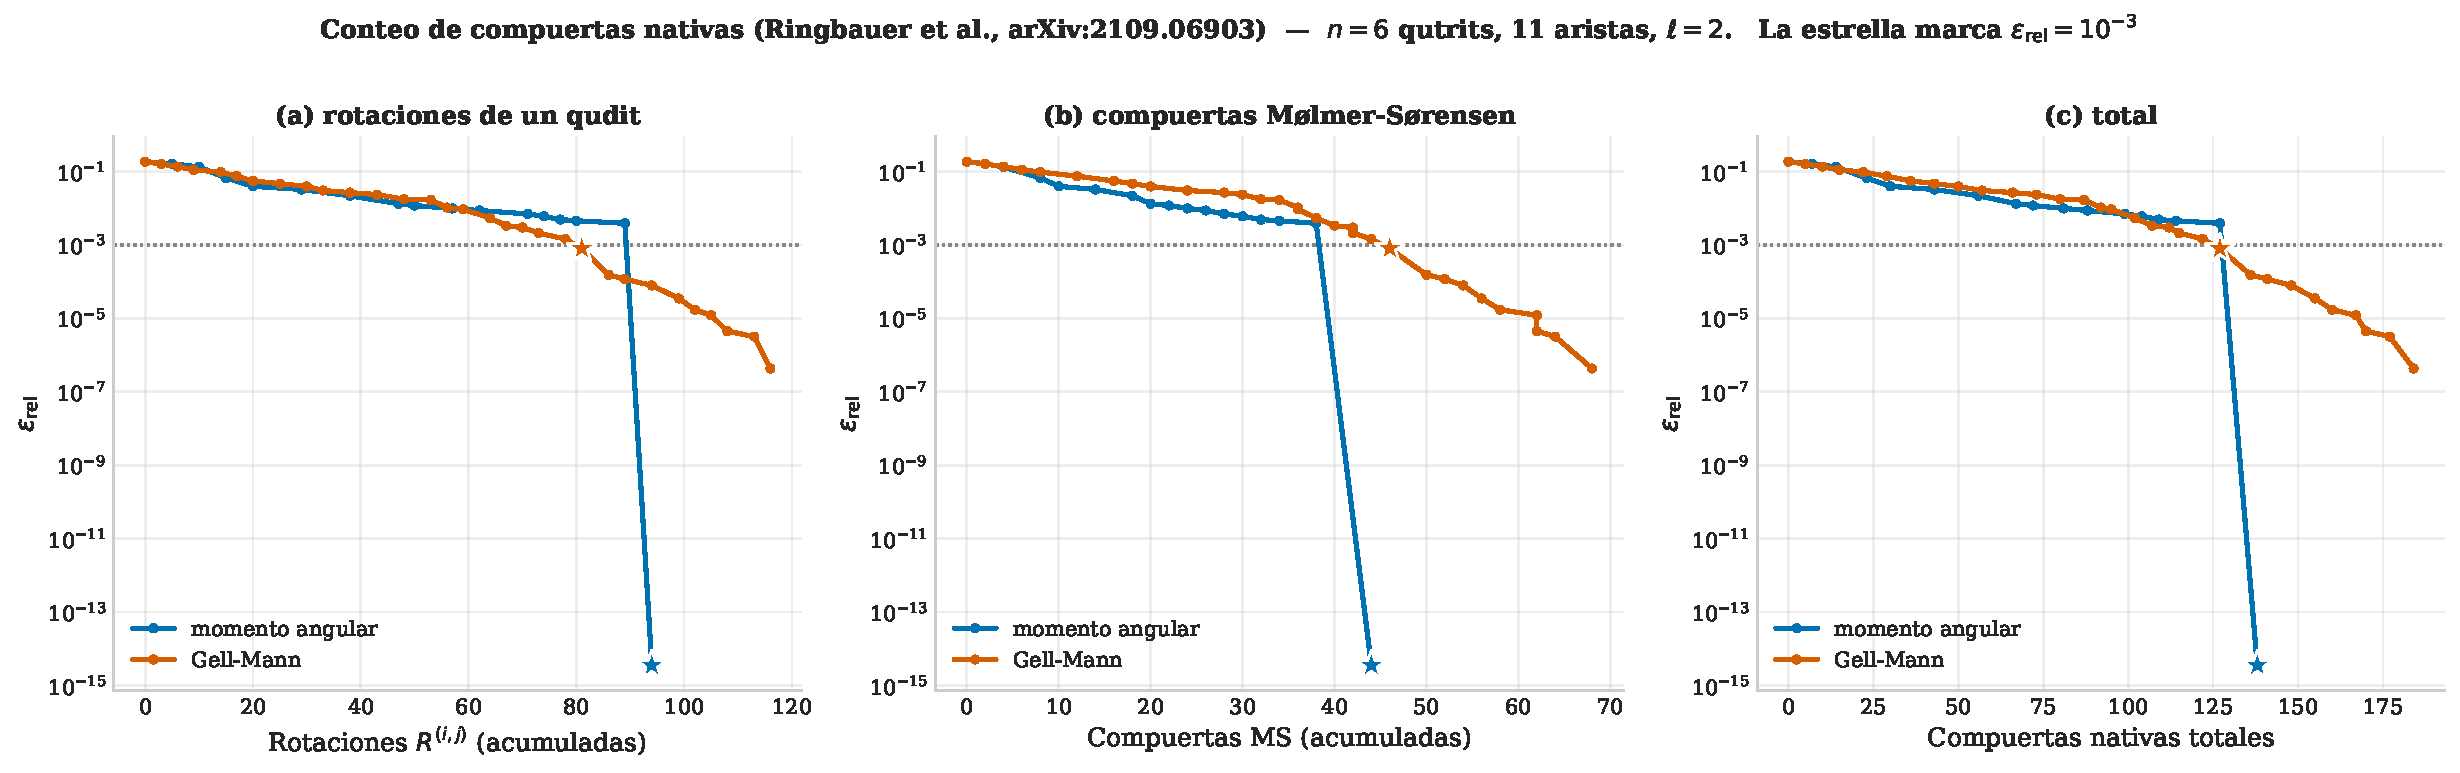
\includegraphics[width=\textwidth]{bp_compuertas_nativas.pdf}
\caption{Error relativo contra compuertas nativas acumuladas, separando
rotaciones de un qudit, compuertas MS y el total. La estrella marca
$\epsilon_{\rm rel}=10^{-3}$.}
\label{fig:compuertas}
\end{figure}

El resultado \textbf{invierte parcialmente} la conclusión de la sección
anterior. A igual precisión $\epsilon_{\rm rel}<10^{-3}$:

\begin{center}
\begin{tabular}{lrrrr}
\toprule
Base & Parámetros & $R^{(i,j)}$ & MS & Total \\
\midrule
Momento angular & 16 & 94 & 44 & 138 \\
Gell-Mann & 21 & \textbf{81} & 46 & \textbf{127} \\
\bottomrule
\end{tabular}
\end{center}

Gell-Mann usa más parámetros y prácticamente las mismas compuertas MS, pero 13
rotaciones de un qudit menos, y termina con un 8\,\% menos de compuertas
totales. La causa está en el promedio de rotaciones de dos niveles por
generador: $3.87$ frente a $5.88$. Las matrices de Gell-Mann casi coinciden con
la compuerta nativa --- $\lambda_3,\lambda_8$ son diagonales y el resto actúa
dentro de un solo par de niveles --- mientras que los monomios angulares
hermitizados son hermíticas $3\times3$ genéricas.

\paragraph{Un costo oculto del pool angular.} Cuando dos o más sitios tienen
factor local no hermítico, $(O+O^\dagger)/2$ deja de ser un producto tensorial
y pasa a ser una suma de dos productos que no conmutan; la construcción de
escalera no aplica y haría falta trotterizar. En el ansatz medido, 2 de 16
generadores angulares caen en ese caso, y ninguno de los de Gell-Mann. Ese
costo extra no está incluido en las 138 compuertas de la tabla.

\paragraph{Qué es exacto y qué es modelo.} Es exacto el número de rotaciones de
dos niveles de cada factor local, calculado de la matriz contando qué pares de
niveles conecta. Es modelo la escalera de $2(w-1)$ compuertas MS, extrapolada
de la construcción de qubits. El ancla más cercana que da ese trabajo es su
compuerta de intercambio controlado, que se descompone en dos MS de dos
niveles independientemente de la dimensión y coincide entonces con el caso
$w=2$; la extensión a $w>2$ es nuestra y no corresponde a un circuito
compilado.

\paragraph{Matiz.} El pool angular sí alcanza precisión de máquina, y el de
Gell-Mann se queda en $4\times10^{-7}$ tras 30 parámetros. La ventaja en
compuertas vale en el régimen de precisión moderada --- que es el relevante
para hardware NISQ --- pero no es universal.

\section{Limitaciones}

Conviene ser explícito sobre qué \emph{no} se demostró:

\begin{itemize}
\item \textbf{El barrido es en profundidad, no en tamaño.} Todos los
diagnósticos se hicieron a $n=6$ qutrits fijo (o hasta $n=6$ para la QFIM). La
definición estricta de \emph{barren plateau} es sobre el escalamiento con el
número de qudits, $\mathrm{Var}(\partial_\theta E)\sim e^{-\alpha n}$. Cerrar
esa afirmación exige repetir el diagnóstico para $n=4,5,6,7$ y ajustar la
exponencial en $n$.

\item \textbf{Falta un control positivo.} Una curva plana sólo es informativa
si el diagnóstico es capaz de detectar una meseta cuando la hay. Sin un ansatz
que sí sufra \emph{barren plateaus} --- por ejemplo el \emph{hardware-efficient}
para qutrits --- queda abierta la objeción de que la métrica sea insensible.
Esto es especialmente relevante porque existe literatura que sostiene que los
\emph{barren plateaus} se \emph{amplifican} con la dimensión del qudit
(Friedrich, de Souza Farias \& Maziero, \emph{Quantum Machine Intelligence},
2025), lo que iría en contra del resultado aquí reportado.

\item \textbf{Simulación exacta, sin ruido.} No hay ruido de muestreo ni de
hardware. Un gradiente pequeño pero no nulo puede ser inobservable con un
número finito de mediciones.

\item \textbf{Un grafo por configuración.} Las conclusiones se apoyan en
instancias individuales. La comparación de pools, en particular, necesita
repetirse sobre el ensemble de 300 grafos disponible antes de afirmarse.

\item \textbf{El DLA quedó incompleto.} Sólo se cerró para $n=2$ y $n=3$.
\end{itemize}

\section{Trabajo pendiente}

En orden de valor:

\begin{enumerate}
\item \textbf{Control positivo.} Implementar un ansatz \emph{hardware-efficient}
para qutrits que aproxime un 2-design, y mostrar su varianza colapsando junto a
la del pool contradiabático que no colapsa.

\item \textbf{Varianza frente a $n$.} El test canónico: muestrear
$\boldsymbol\theta$ uniforme, calcular $\partial_\theta E$, y ajustar
$\log\mathrm{Var}$ contra $n$ para $n=3,\dots,7$. Es barato porque no requiere
optimizar.

\item \textbf{Discriminar la causa del resultado negativo.} Agregar al pool de
Gell-Mann las $8n$ rotaciones de un solo sitio. Si el hueco se cierra, la causa
era la ausencia de operadores locales; si no, era el carácter atómico de los
strings. \emph{(En ejecución.)}

\item \textbf{Una tercera base.} Heisenberg-Weyl ($X^aZ^b$ generalizadas)
aísla las dos variables: es una descomposición fina como Gell-Mann pero con
elementos no hermíticos como la angular. \emph{(En ejecución.)}

\item \textbf{Ensemble.} Repetir la comparación de pools sobre los 300 grafos
disponibles. El código está preparado con guardado incremental y reanudación.

\item \textbf{Completar el DLA} para $n=4$ y, si es viable, $n=5$.
\end{enumerate}

\section*{Reproducibilidad}

Todo el código vive en el repositorio del proyecto:

\begin{center}
\begin{tabular}{ll}
\toprule
Archivo & Contenido \\
\midrule
\texttt{funciones/utilidades\_bp.py} & motor del experimento, QFIM, DLA, figuras \\
\texttt{funciones/utilidades\_gellmann.py} & álgebra y pool en base de Gell-Mann \\
\texttt{funciones/utilidades\_heisenberg.py} & álgebra y pool en base de Heisenberg-Weyl \\
\texttt{cluster/main\_bp.py} & corridas individuales, con checkpoint por iteración \\
\texttt{cluster/main\_ensemble\_pools.py} & comparación sobre un ensemble, reanudable \\
\texttt{cuadernillos/barren\_plateaus.ipynb} & cuadernillo con todo el análisis \\
\bottomrule
\end{tabular}
\end{center}

\noindent
Los resultados numéricos completos quedan en \texttt{resultados/json/} y las
figuras en \texttt{resultados/images/}. Las corridas usan semilla fija; se
verificó que los resultados son idénticos en modo serial y paralelo.

\end{document}
